\iffalse
\let\negmedspace\undefined
\let\negthickspace\undefined
\documentclass[journal,12pt,twocolumn]{IEEEtran}
\usepackage{cite}
\usepackage{amsmath,amssymb,amsfonts,amsthm}
\usepackage{algorithmic}
\usepackage{graphicx}
\usepackage{textcomp}
\usepackage{xcolor}
\usepackage{txfonts}
\usepackage{listings}
\usepackage{enumitem}
\usepackage{mathtools}
\usepackage{gensymb}
\usepackage{comment}
\usepackage[breaklinks=true]{hyperref}
\usepackage{tkz-euclide} 
\usepackage{listings}
\usepackage{gvv}  
\usepackage{tikz}
\usepackage{circuitikz} 
\usepackage{caption}

\def\inputGnumericTable{}                                
\usepackage[latin1]{inputenc}                 
\usepackage{color}                            
\usepackage{array}                            
\usepackage{longtable}                        
\usepackage{calc}                            
\usepackage{multirow}                      
\usepackage{hhline}                           
\usepackage{ifthen}                          
\usepackage{lscape}
\usepackage{amsmath}
\newtheorem{theorem}{Theorem}[section]
\newtheorem{problem}{Problem}
\newtheorem{proposition}{Proposition}[section]
\newtheorem{lemma}{Lemma}[section]
\newtheorem{corollary}[theorem]{Corollary}
\newtheorem{example}{Example}[section]
\newtheorem{definition}[problem]{Definition}
\newcommand{\BEQA}{\begin{eqnarray}}
\newcommand{\EEQA}{\end{eqnarray}}
\newcommand{\define}{\stackrel{\triangle}{=}}
\theoremstyle{remark}
\newtheorem{rem}{Remark}

\begin{document}
\title{}
\author{Sasa Mardi, EE23BTECH11222}
\date{}
\maketitle
\textbf{Question 11.9.3-19:} Find the sum of the products of the corresponding terms of the sequences $2, 4, 8, 16, 32$ and $128, 32, 8, 2, \frac{1}{2}$.\\
\\
\solution
\fi
\begin{table}[h!]
    \centering
    \caption{Input Parameters}
    \label{tab.11.9.3.19:1}
    \begin{tabular}{ | c | c | c | }
        \hline
        Parameter & Value & Description \\
        \hline
        $x_1(n)$ & $2, 4, 8, 16, 32$ &  Sequence 1 \\
        \hline
        $x_2(n)$ & $128, 32, 8, 2, \frac{1}{2}$ &  Sequence 2 \\
        \hline
        $y(n)$ & - &  Sum of the Products \\
        \hline
    \end{tabular}
\end{table}\\
Define the sequences as follows:\\
\begin{align}
&\text{Sequence 1: } x_1(n) = 2(2)^nu(n) \\
&\text{Sequence 2: } x_2(n) = 128\left(\frac{1}{4}\right)^nu(n)
\end{align}
\begin{align}
x(n) &= x_1(n)x_2(n) \\
x(n) &= \left(\frac{256}{2^{n}}\right)u(n)
\end{align}
\textbf{Z-Transform:}
The Z-transform of a sequence \( x(n) \) is:
\begin{align}
X(z) &= \frac{256}{1 - \frac{z^{-1}}{2}}    \quad |z| > \frac{1}{2}
\end{align}
\begin{align}
Let, y(n) &= x(n)*u(n) \\
 Y(z) &= X(z)U(z) \\
 &= \left(\frac{256}{1 - \frac{z^{-1}}{2}}\right)\left(\frac{1}{1 - z^{-1}}\right)\\
 &= \frac{-256}{1 - \frac{z^{-1}}{2}} + \frac{512}{1 - z^{-1}}
\end{align}

\textbf{Inverse of Z Transform of Y(z):} \\
\begin{align}
y(n) &= \left[\frac{-256}{2^{n}} + \frac{512}{1}\right]u(n)
\end{align}
\begin{figure}[h!]
    \centering
    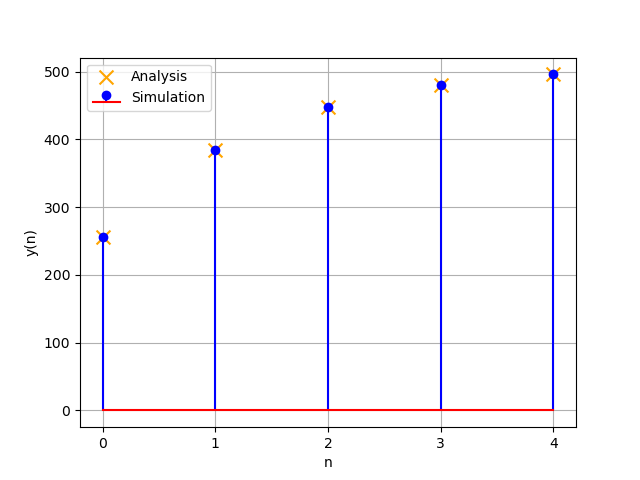
\includegraphics[width=\columnwidth]{ncert-maths/11/9/3/19/figs/fig1.png}
    \caption{Plot of $y(n)$ vs $n$}
    \label{fig.11.9.3.19:1}
\end{figure}
As, n = 4, sum = 496. \\
This gives us the sum of the products of corresponding terms, which is 496.
